\documentclass[11pt, letterpaper, includehead]{article}

%%%%%%%%%%%%%%%%%%%%% Pre-document %%%%%%%%%%%%%%%%%%%%%
\usepackage{fancyhdr}  % Allow for headers
\usepackage{graphicx}  % Allow for figures 
\usepackage{float}     % Allow for figure inserted in specified location
\usepackage{textcomp}  % Trade mark symbol
\usepackage{multicol}
\usepackage{amsmath}

\setlength{\parindent}{0pt} % Remove auto paragraph indents

% Get rid of those big ass margins
\usepackage[margin=1in]{geometry}

% Table cell formatting
\setlength{\arrayrulewidth}{0.25mm}
\setlength{\tabcolsep}{11pt}
\renewcommand{\arraystretch}{1.2}

\begin{document}

%%%%%%%%%%%%%%%%%%%%% Title Page %%%%%%%%%%%%%%%%%%%%%
\begin{titlepage}
  \begin{center}
    \Huge{\textbf{Lab 3}}\\
    \Huge{Vectors}
    \vfill
    \begin{figure}[H] % H makes the figure insert at the position in the document
      \centering
      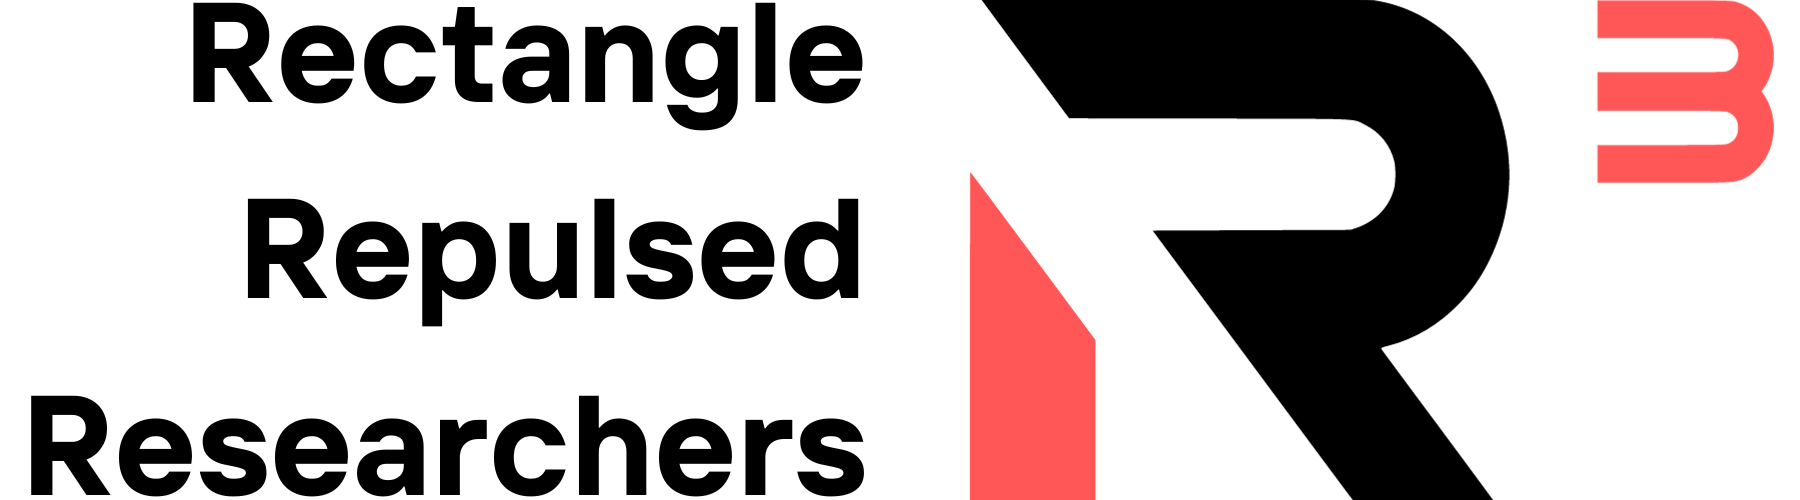
\includegraphics[width=6cm]{../logo.png}
    \end{figure}
    \Large{\textbf{Name}}\\
      \vspace{0.25cm}
      \large{Julian Barossi, Liam Gilligan}\\
      \vspace{0.25cm}
      \normalsize
      \today
  \end{center}
\end{titlepage}

%%%%%%%%%%%%%%%%%%%%% TABLE OF CONTENTS %%%%%%%%%%%%%%%%%%%%%
\tableofcontents
\pagebreak % Move to next page

% Add a nice fancy header
\pagestyle{fancy}
\fancyhead{}
\fancyhead[C]{\textbf{Lab 3:} Vectors}

\pagebreak 

%%%%%%%%%%%%%%%%%%%%% ADDING TWO VECTORS %%%%%%%%%%%%%%%%%%%%%
\section{Adding Two Vectors} % 1

%%%%%%%%%%%%%%%%%%%%% GIVEN VECTORS %%%%%%%%%%%%%%%%%%%%%
\subsection{Given vectors} % 1.1
The force vectors given were $35g$ at an angle of $60^{\circ}$ and $55g$ at an angle of $160^{\circ}$

\subsubsection{Find components} % 1.1.1
The $x$ and $y$ components of a vector are defined as a the amount the vector 
points along each axis. Vector components can be calculated using the Southern 
California Approach\textsuperscript{TM} or SOCA in which the component opposite to
$\theta$ is found by $\pm F \sin\theta$ and the adjacent to $\theta$ is $\pm F \cos\theta$

\begin{multicols}{2}
  \centering{\textbf{Force 1}}
  $$F_1 = mg$$
  $$F_1 = 35g \cdot \frac{1kg}{1000g} \cdot 9.80m/s^2$$
  $$F_1 = 0.343N$$

  $$F_{1_x} = F_1\cos\theta$$
  $$F_{1_x} = 0.343N\cos60^{\circ}$$
  $$F_{1_x} = 0.1715N \approx 0.172N$$
  $$\boxed{F_{1_x} = 0.172N}$$

  $$F_{1_y} = F_1\sin\theta$$
  $$F_{1_y} = 0.343N\sin60^{\circ}$$
  $$F_{1_y} = 0.2970467...N \approx 0.297N$$
  $$\boxed{F_{1_y} = 0.297N}$$

  \columnbreak
  \centering{\textbf{Force 2}}
  $$F_2 = mg$$
  $$F_2 = 55g \cdot \frac{1kg}{1000g} \cdot 9.80m/s^2$$
  $$F_2 = 0.539N$$

  $$F_{2_x} = F_2\cos\theta$$
  $$F_{2_x} = 0.539N\cos160^{\circ}$$
  $$F_{2_x} = -0.506494...N \approx -0.506N$$
  $$\boxed{F_{2_x} = -0.506N}$$

  $$F_{2_y} = F_1\sin\theta$$
  $$F_{2_y} = 0.539N\sin160^{\circ}$$
  $$F_{2_y} = 0.184348...N \approx 0.184N$$
  $$\boxed{F_{2_y} = 0.184N}$$
\end{multicols}

\subsubsection{Two forces to balance the net force} % 1.1.2
Two forces which balance the net force ($\vec{F}_{net}$) can be found by calculating the sum of 
the original and vectors. Then apply the opposite of the the sum vector's $x$ and $y$ components to balance.
% $$\vec{F}_{net} = \vec{F}_{1} + \vec{F}_{2}$$
$$R_x = F_{1_x} + F_{2_x} = 0.1715N + (-0.506494N) = -0.334994N \approx \boxed{-0.335N}$$
$$R_y = F_{1_y} + F_{2_y} = 0.2970467N + 0.184348N = 0.4813947N \approx \boxed{0.481N}$$
$0.335N$ should be applied in the positive $x$ and $0.481N$ in the negative $y$.

\subsubsection{Was the prediction correct} % 1.1.3
The predicted forces balanced out the original opposing forces. 

\subsubsection{Single forces to balance the net force} % 1.1.4
A vector which has the same magnitude of the sum of $\vec{F_1}$ and $\vec{F_2}$ 
and opposite direction would balance the forces.\\
Magnitude:
$$R = \sqrt{R_x^2 + R_y^2} = \sqrt{(-0.334994N)^2 + (0.4813947N)^2} = 0.586482023N \approx \boxed{0.586N}$$
Direction:
$$\theta = \arctan \left( \frac{R_y}{R_x} \right) + 180^{\circ} \text{ if } R_x < 0$$
$$\theta = \arctan \left( \frac{0.4813947N}{-0.334994N} \right) + 180^{\circ}$$
$$\theta = 124.8333695^{\circ} \approx {125^{\circ}}$$
$$\theta_{opp} = 125^{\circ} + 180^{\circ} = \boxed{305^{\circ}}$$

The force vector required to to balance $\vec{F_1}$ and $\vec{F_2}$ is
$R = 0.586N \text{ at } \theta = 305^{\circ}$

\subsubsection{Was the prediction correct} % 1.1.5
The predicted force balanced out the original opposing forces. 

%%%%%%%%%%%%%%%%%%% CHOSEN VECTORS %%%%%%%%%%%%%%%%%%%%%
\subsection{Chosen vectors} % 1.2
The force vectors chosen were $105g$ at an angle of $87^{\circ}$ and $15g$ at an angle of $48^{\circ}$

\subsubsection{Find components} % 1.2.1
\begin{multicols}{2}
  \centering{\textbf{Force 1}}
  $$F_1 = mg$$
  $$F_1 = 105g \cdot \frac{1kg}{1000g} \cdot 9.80m/s^2$$
  $$F_1 = 1.029N$$

  $$F_{1_x} = F_1\cos\theta$$
  $$F_{1_x} = 1.029N\cos87^{\circ}$$
  $$F_{1_x} = 0.053853699...N \approx 0.0539N$$
  $$\boxed{F_{1_x} = 0.0539N}$$

  \columnbreak
  \centering{\textbf{Force 2}}
  $$F_2 = mg$$
  $$F_2 = 15g \cdot \frac{1kg}{1000g} \cdot 9.80m/s^2$$
  $$F_2 = 0.147N$$

  $$F_{2_x} = F_2\cos\theta$$
  $$F_{2_x} = 0.147N\cos48^{\circ}$$
  $$F_{2_x} = 0.098362199...N \approx 0.0984N$$
  $$\boxed{F_{2_x} = 0.0984N}$$
 
\end{multicols}

\begin{multicols}{2}

  $$F_{1_y} = F_1\sin\theta$$
  $$F_{1_y} = 1.029N\sin87^{\circ}$$
  $$F_{1_y} = 1.027589791...N \approx 1.03N$$
  $$\boxed{F_{1_y} = 1.03N}$$

  \columnbreak
  $$F_{2_y} = F_2\sin\theta$$
  $$F_{2_y} = 0.147N\sin48^{\circ}$$
  $$F_{2_y} = 0.109242289...N \approx 0.109N$$
  $$\boxed{F_{2_y} = 0.109N}$$
 
\end{multicols}

\subsubsection{Two forces to balance the net force} % 1.2.2
$$R_x = F_{1_x} + F_{2_x} = 0.053853699N + 0.098362199N = 0.1522158984N \approx \boxed{0.152N}$$
$$R_y = F_{1_y} + F_{2_y} = 1.027589791N + 0.109242289N = 1.13683208N \approx \boxed{1.137N}$$
$0.152N$ should be applied in the negative $x$ and $1.137N$ in the negative $y$.

\subsubsection{Was the prediction correct} % 1.2.3
The predicted forces balanced out the original opposing forces. 

\subsubsection{Single force to balance the net force} % 1.2.4
Magnitude:
$$R = \sqrt{R_x^2 + R_y^2} = \sqrt{(0.1522158984N)^2 + (1.13683208N)^2} = 1.14697727N \approx \boxed{1.15N}$$
Direction:
$$\theta = \arctan \left( \frac{R_y}{R_x} \right) + 180^{\circ} \text{ if } R_x < 0$$
$$\theta = \arctan \left( \frac{1.13683208N}{0.1522158984N} \right)$$
$$\theta = 82.373775148^{\circ} \approx {82.4^{\circ}}$$
$$\theta_{opp} = 82.4^{\circ} + 180^{\circ} = \boxed{262^{\circ}}$$
The force vector required to to balance $\vec{F_1}$ and $\vec{F_2}$ is
$R = 1.15N \text{ at } \theta = 262^{\circ}$

\subsubsection{Was the prediction correct} % 1.2.5
The predicted force balanced out the original opposing forces. 

%%%%%%%%%%%%%%%%%%% ADDING THREE VECTORS %%%%%%%%%%%%%%%%%%%%%
\section{Adding three vectors} % 2

%%%%%%%%%%%%%%%%%%%%% GIVEN VECTORS %%%%%%%%%%%%%%%%%%%%%
\subsection{Given vectors} % 2.1
The force vectors given were $35g$ at an angle of $30^{\circ}$, $65g$ at an angle of $110^{\circ}$ and 
$45g$ at $195^{\circ}$
\pagebreak

\subsubsection{Find components} % 2.1.1
\begin{multicols}{3}
  \centering{\textbf{Force 1}}
  $$F_1 = mg$$
  $$F_1 = 35g \cdot \frac{1kg}{1000g} \cdot 9.80m/s^2$$
  $$F_1 = 0.343N$$

  $$F_{1_x} = F_1\cos\theta$$
  $$F_{1_x} = 0.343N\cos30^{\circ}$$
  $$F_{1_x} = 0.297047...N \approx 0.297N$$
  $$\boxed{F_{1_x} = 0.297N}$$

  $$F_{1_y} = F_1\sin\theta$$
  $$F_{1_y} = 0.343N\sin30^{\circ}$$
  $$F_{1_y} = 0.1715...N \approx 0.172N$$
  $$\boxed{F_{1_y} = 0.172N}$$

  \columnbreak
  \centering{\textbf{Force 2}}
  $$F_2 = mg$$
  $$F_2 = 65g \cdot \frac{1kg}{1000g} \cdot 9.80m/s^2$$
  $$F_2 = 0.637N$$

  $$F_{2_x} = F_1\cos\theta$$
  $$F_{2_x} = 0.637N\cos110^{\circ}$$
  $$F_{2_x} = -0.217867...N \approx -0.218N$$
  $$\boxed{F_{2_x} = -0.218N}$$

  $$F_{2_y} = F_1\sin\theta$$
  $$F_{2_y} = 0.637N\sin110^{\circ}$$
  $$F_{2_y} = 0.598584...N \approx 0.599N$$
  $$\boxed{F_{2_y} = 0.599N}$$

  \columnbreak
  \centering{\textbf{Force 3}}
  $$F_3 = mg$$
  $$F_3 = 45g \cdot \frac{1kg}{1000g} \cdot 9.80m/s^2$$
  $$F_3 = 0.441N$$

  $$F_{3_x} = F_1\cos\theta$$
  $$F_{3_x} = 0.441N\cos195^{\circ}$$
  $$F_{3_x} = -0.425973...N \approx -0.426N$$
  $$\boxed{F_{1_x} = -0.426N}$$

  $$F_{3_y} = F_1\sin\theta$$
  $$F_{3_y} = 0.441N\sin195^{\circ}$$
  $$F_{3_y} = -0.1141391...N \approx -0.114N$$
  $$\boxed{F_{3_y} = -0.114N}$$
 
\end{multicols}

\subsubsection{Single force to balance the net force} % 2.1.2
Components:
$$R_x = F_{1_x} + F_{2_x} + F_{3_x} = 0.297047N + (-0.217867N) + (-0.425973N) = -0.346793N \approx \boxed{-0.347N} $$
$$R_y = F_{1_y} + F_{2_y} + F_{3_y} = 0.1715N + 0.598584N + (-0.1141391N) = 0.6559449N \approx \boxed{0.656N} $$
Magnitude:
$$R = \sqrt{R_x^2 + R_y^2} = \sqrt{(-0.346793N)^2 + (0.6559449N)^2} = 0.741976...N \approx \boxed{0.742N}$$
Direction:
$$\theta = \arctan \left( \frac{R_y}{R_x} \right) + 180^{\circ} \text{ if } R_x < 0$$
$$\theta = \arctan \left( \frac{0.6559449N}{-0.346793N} \right) + 180^{\circ}$$
$$\theta = 117.8650623^{\circ} \approx {118^{\circ}}$$
$$\theta_{opp} = 118^{\circ} + 180^{\circ} = \boxed{298^{\circ}}$$

The force vector required to to balance $\vec{F_1}$, $\vec{F_2}$, and $\vec{F_3}$ is
$R = 0.742N \text{ at } \theta = 298^{\circ}$

\subsubsection{Was the prediction correct} % 2.1.3
The predicted forces balanced out the original opposing forces. 

%%%%%%%%%%%%%%%%%%%%% CHOSEN VECTORS %%%%%%%%%%%%%%%%%%%%%
\subsection{Chosen vectors} % 2.2
The force vectors chosen were $17g$ at an angle of $22^{\circ}$, $45g$ at an angle of $171^{\circ}$, and $150g$ at $150^{\circ}$

\subsubsection{Find components} % 2.2.1
\begin{multicols}{3}
  \centering{\textbf{Force 1}}
  $$F_1 = mg$$
  $$F_1 = 17g \cdot \frac{1kg}{1000g} \cdot 9.80m/s^2$$
  $$F_1 = 0.1666N$$

  $$F_{1_x} = F_1\cos\theta$$
  $$F_{1_x} = 0.1666N\cos22^{\circ}$$
  $$F_{1_x} = 0.154469...N \approx 0.154N$$
  $$\boxed{F_{1_x} = 0.154N}$$

  $$F_{1_y} = F_1\sin\theta$$
  $$F_{1_y} = 0.1666N\sin22^{\circ}$$
  $$F_{1_y} = 0.0624095...N \approx 0.0624N$$
  $$\boxed{F_{1_y} = 0.0624N}$$

  \columnbreak
  \centering{\textbf{Force 2}}
  $$F_2 = mg$$
  $$F_2 = 45g \cdot \frac{1kg}{1000g} \cdot 9.80m/s^2$$
  $$F_2 = 0.441N$$

  $$F_{2_x} = F_1\cos\theta$$
  $$F_{2_x} = 0.441N\cos271^{\circ}$$
  $$F_{2_x} = 0.00769651N \approx 0.00770N$$
  $$\boxed{F_{2_x} = 0.00770N}$$

  $$F_{2_y} = F_1\sin\theta$$
  $$F_{2_y} = 0.441N\sin271^{\circ}$$
  $$F_{2_y} = -0.440933...N \approx -0.441N$$
  $$\boxed{F_{2_y} = -0.441N}$$

  \columnbreak
  \centering{\textbf{Force 3}}
  $$F_3 = mg$$
  $$F_3 = 150g \cdot \frac{1kg}{1000g} \cdot 9.80m/s^2$$
  $$F_3 = 1.47N$$

  $$F_{3_x} = F_1\cos\theta$$
  $$F_{3_x} = 1.47N\cos150^{\circ}$$
  $$F_{3_x} = -1.273057...N \approx -1.27N$$
  $$\boxed{F_{1_x} = -1.27N}$$

  $$F_{3_y} = F_1\sin\theta$$
  $$F_{3_y} = 1.47N\sin150^{\circ}$$
  $$F_{3_y} = 0.735N$$
  $$\boxed{F_{3_y} = 0.735N}$$
 
\end{multicols}

\subsubsection{Single forces to balance the net force} % 2.2.2
Components:
$$R_x = F_{1_x} + F_{2_x} + F_{3_x} = 0.154469N + 0.00769651N + (-1.273057N) = -1.11089N \approx \boxed{-1.111N} $$
$$R_y = F_{1_y} + F_{2_y} + F_{3_y} = 0.0624095N + (-0.440933N) + 0.735N = 0.3565N \approx \boxed{0.357N} $$
Magnitude:
$$R = \sqrt{R_x^2 + R_y^2} = \sqrt{(-1.11089N)^2 + (0.3565N)^2} = 1.1667...N \approx \boxed{1.17N}$$
Direction:
$$\theta = \arctan \left( \frac{R_y}{R_x} \right) + 180^{\circ} \text{ if } R_x < 0$$
$$\theta = \arctan \left( \frac{0.3565N}{-1.11089N} \right) + 180^{\circ}$$
$$\theta = 162.208\dots^{\circ} \approx {162^{\circ}}$$
$$\theta_{opp} = 162^{\circ} + 180^{\circ} = \boxed{342^{\circ}}$$

The force vector required to to balance $\vec{F_1}$, $\vec{F_2}$, and $\vec{F_3}$ is
$R = 1.17N \text{ at } \theta = 342^{\circ}$

\subsubsection{Was the prediction correct} % 2.2.3
The predicted forces balanced out the original opposing forces. 

%%%%%%%%%%%%%%%%%%% BURIED TREASURE %%%%%%%%%%%%%%%%%%%%%
\section{Hunt for Buried Treasure} % 3
\subsection{Game A} % 3.1
\begin{enumerate}
  \item From the starting point, first move 20.83 cm at 147°.
  \item Next, travel 1.5 x 10 5 $\mu$ due west.
  \item Finally, go 0.489 m at an angle of 32.2° above the +x-axis.
\end{enumerate}

\begin{multicols}{3}
  \centering{\textbf{Part 1}}
  $$r_1 = 20.83cm\text{ at }147^{\circ}$$
  $$r_{1_x} = 20.83cm\cos147^{\circ}$$
  $$r_{1_x} = -17.469cm \approx -17.47cm$$
  $$r_{1_y} = 20.83cm\sin147^{\circ}$$
  $$r_{1_y} = 11.3448cm \approx 11.34cm$$
  \columnbreak

  \centering{\textbf{Part 2}}
  $$r_2 = 150000\mu m\text{ due west }$$
  $$r_2 = 150000\mu m\cdot\frac{1cm}{10000\mu m}\text{ west }$$
  $$r_2 = 15cm\text{ at }180^{\circ}$$
  $$r_{2_x} = 15cm\cos180^{\circ}$$
  $$r_{2_x} = -15cm$$
  $$r_{2_y} = 20.83cm\sin180^{\circ}$$
  $$r_{2_y} = 0cm$$

  \columnbreak
  \centering{\textbf{Part 3}}
  $$r_3 = 0.489m\text{ at }32.2^{\circ}$$
  $$r_3 = 0.489m\cdot\frac{100cm}{1m}\text{ at }32.2^{\circ}$$
  $$r_3 = 48.9cm\text{ at }32.2^{\circ}$$
  $$r_{3_x} = 48.9cm\cos32.2^{\circ}$$
  $$r_{3_x} = 41.3788cm \approx 41.38cm$$
  $$r_{3_y} = 48.9cm\sin32.2^{\circ}$$
  $$r_{3_y} = 26.0576cm \approx 26.06cm$$

\end{multicols}

\hspace{0.5cm}

\begin{multicols}{2}
  \centering\textbf{x-component}
  $$r_x = r_{1_x} + r_{2_x} + r_{3_x}$$
  $$r_x = -17.47cm + -15cm + 41.38cm$$
  $$r_x = 8.909337894cm \approx{8.91cm}$$
  $$\boxed{r_x = {8.91cm}}$$

  \columnbreak
  \centering\textbf{y-component}
  $$r_y = r_{1_y} + r_{2_y} + r_{3_y}$$
  $$r_y = 11.34cm +  0cm + 26.06cm$$
  $$r_y = 37.402480999cm \approx 37.4cm$$
  $$\boxed{r_y = 37.4cm}$$
  
\end{multicols}

\subsection{Game B} % 3.2
\begin{enumerate}
  \item From the starting point, first move so that your displacement is
  \\ $r = (+0.28m)\hat\imath+(7.0 \times 10^2mm)\hat\jmath$
  \item Next, walk at $1.50 mi/hr$ due north for $ 0.40 s$.
  \item Finally, walk $86.9 cm$ at $41.2^{\cdot}$ south of west
\end{enumerate}

\begin{multicols}{2}
  \centering{\textbf{Part 1}}
  $$r_1 = (+0.28m)\hat\imath +(7.0\times10^2mm)\hat\jmath$$
  $$r_{1_x} = 0.28m\cdot\frac{100cm}{1m}$$
  $$r_{1_x} = 28cm$$
  $$r_{1_y} = 7.0\times10^2mm\cdot\frac{1cm}{10mm}$$
  $$r_{1_y} = 70cm$$

  \columnbreak
  \centering{\textbf{Part 2}}
  $$r_2 = 1.50\cdot\frac{mi}{hr} \text{ due north for }0.40s$$
  $$r_2 = 1.50\cdot\frac{mi}{hr}\cdot\frac{1609m}{1mi}\cdot\frac{100cm}{1m}\cdot\frac{1hr}{3600s}\cdot0.40s$$
  $$r_2 = 26.8cm$$
  $$r_{2_x} = 0cm$$
  $$r_{2_y} = 26.8cm$$
\end{multicols}

\hspace{0.5cm}

\centering{\textbf{Part 3}}
$$r_3 = 86.9cm \text{ at } 41.2^{\circ} \text{ south of west}$$
$$r_3 = 86.9cm \text{ at } 221.2^{\circ}$$
$$r_{3_x} = 86.9cm\cdot\cos221.2^{\circ}$$
$$r_{3_x} = -65.384855583cm \approx -65.38cm$$
$$r_{3_y} = 86.9cm\cdot\cos221.2^{\circ}$$
$$r_{3_y} = -57.240114084cm \approx -57.24cm$$

\hspace{0.5cm}

\begin{multicols}{2}
  \centering\textbf{x-component}
  $$r_x = r_{1_x} + r_{2_x} + r_{3_x}$$
  $$r_x = 28cm + 0cm -65.38cm$$
  $$r_x = -37.384855583cm \approx -37.38cm$$
  $$\boxed{r_x = -37.4cm}$$

  \centering\textbf{y-component}
  $$r_y = r_{1_y} + r_{2_y} + r_{3_y}$$
  $$r_y = 70cm + 26.8cm - 57.24cm$$
  $$r_y = 39.559885916cm \approx 39.56cm$$
  $$\boxed{r_y = 39.7cm} $$
\end{multicols}

\pagebreak
\subsection{Game C} % 3.3
\begin{enumerate}
  \item From the starting point, skip $2.7 \times 10-4 km$ northwest.
  \item Next, walk $56.3 cm$ at $\theta = 342^{\circ}$.
  \item Then, walk $1.00 km/day$ west for $1.26$ minutes.
  \item Finally, move $0.552 m$ at $-45.6^{\circ}$.
\end{enumerate}

\begin{multicols}{2}
  \centering{\textbf{Part 1}}
  $$r_1 = 2.7\times10^{-4}km \text{ northwest}$$
  $$r_1 = 2.7\times10^{-4}km \cdot\frac{100000cm}{km}\text{ at }135^{\circ}$$
  $$r_1 = 27cm \text{ at }135^{\circ}$$
  $$r_{1_x} = 27cm\cdot\cos135^{\circ}$$
  $$r_{1_x} = -19.091883092cm \approx -19.09cm$$
  $$r_{1_y} = 27cm\cdot\sin135^{\circ}$$
  $$r_{1_y} = 19.091883092cm \approx 19.09cm$$

  \columnbreak
  \centering{\textbf{Part 2}}
  $$r_2 = 56.3cm \text{ at } 342^{\circ}$$
  $$r_{2_x} = 56.3cm\cdot\cos342^{\circ}$$
  $$r_{2_x} = 53.544481867cm \approx 53.54cm$$
  $$r_{2_y} = 56.3cm\cdot\cos342^{\circ}$$
  $$r_{2_y} = -17.397656783cm \approx -17.40cm$$
\end{multicols}

\hspace{0.5cm}

\begin{multicols}{2}
  \centering{\textbf{Part 3}}
  $$r_3 = 1.00\cdot\frac{km}{day} \text{ west for }1.25min$$
  $$r_3 = 1.00\cdot\frac{km}{day}\cdot\frac{100000cm}{1km}\cdot\frac{1day}{1440min}\text{ west }1.26min\cdot\frac{60s}{1min}$$
  $$r_3 = 87.5cm\text{ at }180^{\circ}$$
  $$r_{3_x} = 87.5cm\cdot\cos180^{\circ}$$
  $$r_{3_x} = -87.5cm$$
  $$r_{3_y} = 87.5cm\cdot\sin180^{\circ}$$
  $$r_{3_y} = 0cm$$

  \columnbreak
  \centering{\textbf{Part 4}}
  $$r_4 = 0.552m \text{ at } -45.6^{\circ}$$
  $$r_4 = 0.552m\cdot\frac{100cm}{1m} \text{ at } -45.6^{\circ}$$
  $$r_4 = 55.2cm \text{ at } 314.4^{\circ}$$
  $$r_{4_x} = 55.2cm\cdot\cos314.4^{\circ}$$
  $$r_{4_x} = 38.621416396cm \approx 38.62cm$$
  $$r_{4_y} = 55.2cm\cdot\sin314.4^{\circ}$$
  $$r_{4_y} = -39.438891916cm \approx -39.44cm$$
\end{multicols}

\hspace{0.5cm}

\begin{multicols}{2}
  \centering{\textbf{x-component}}
  $$r_x = r_{1_x} + r_{2_x} + r_{3_x} + r_{4_x}$$
  $$r_x = -19.09cm -87.5cm + 38.62cm + 38.62cm$$
  $$r_x = -14.425984829cm \approx -14.43cm$$
  $$\boxed{r_x = -14.4cm}$$
  
  \columnbreak
  \centering{\textbf{y-component}}
  $$r_y = r_{1_y} + r_{2_y} + r_{3_y} r_{4_y}$$
  $$r_y = 19.09cm + 0cm -39.44cm -14.43cm$$
  $$r_y= -34.78cm \approx -34.8cm$$
  $$\boxed{r_y = -37.8cm}$$
\end{multicols}

\end{document}